% !TeX root=main.tex

% Different Number of Ports
\begin{figure*}

	\begin{minipage}[b]{.49\textwidth}
		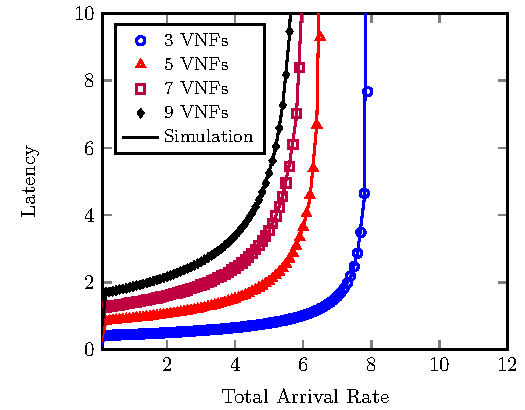
\includegraphics[width=\linewidth]{graphs/diff_lengths}
		\caption{Latency predicted by the model and simulation for a single service with different lengths, $K_i$.}
		\label{fig:length_chain}
	\end{minipage}
	\hfill
	\begin{minipage}[b]{.49\textwidth}
		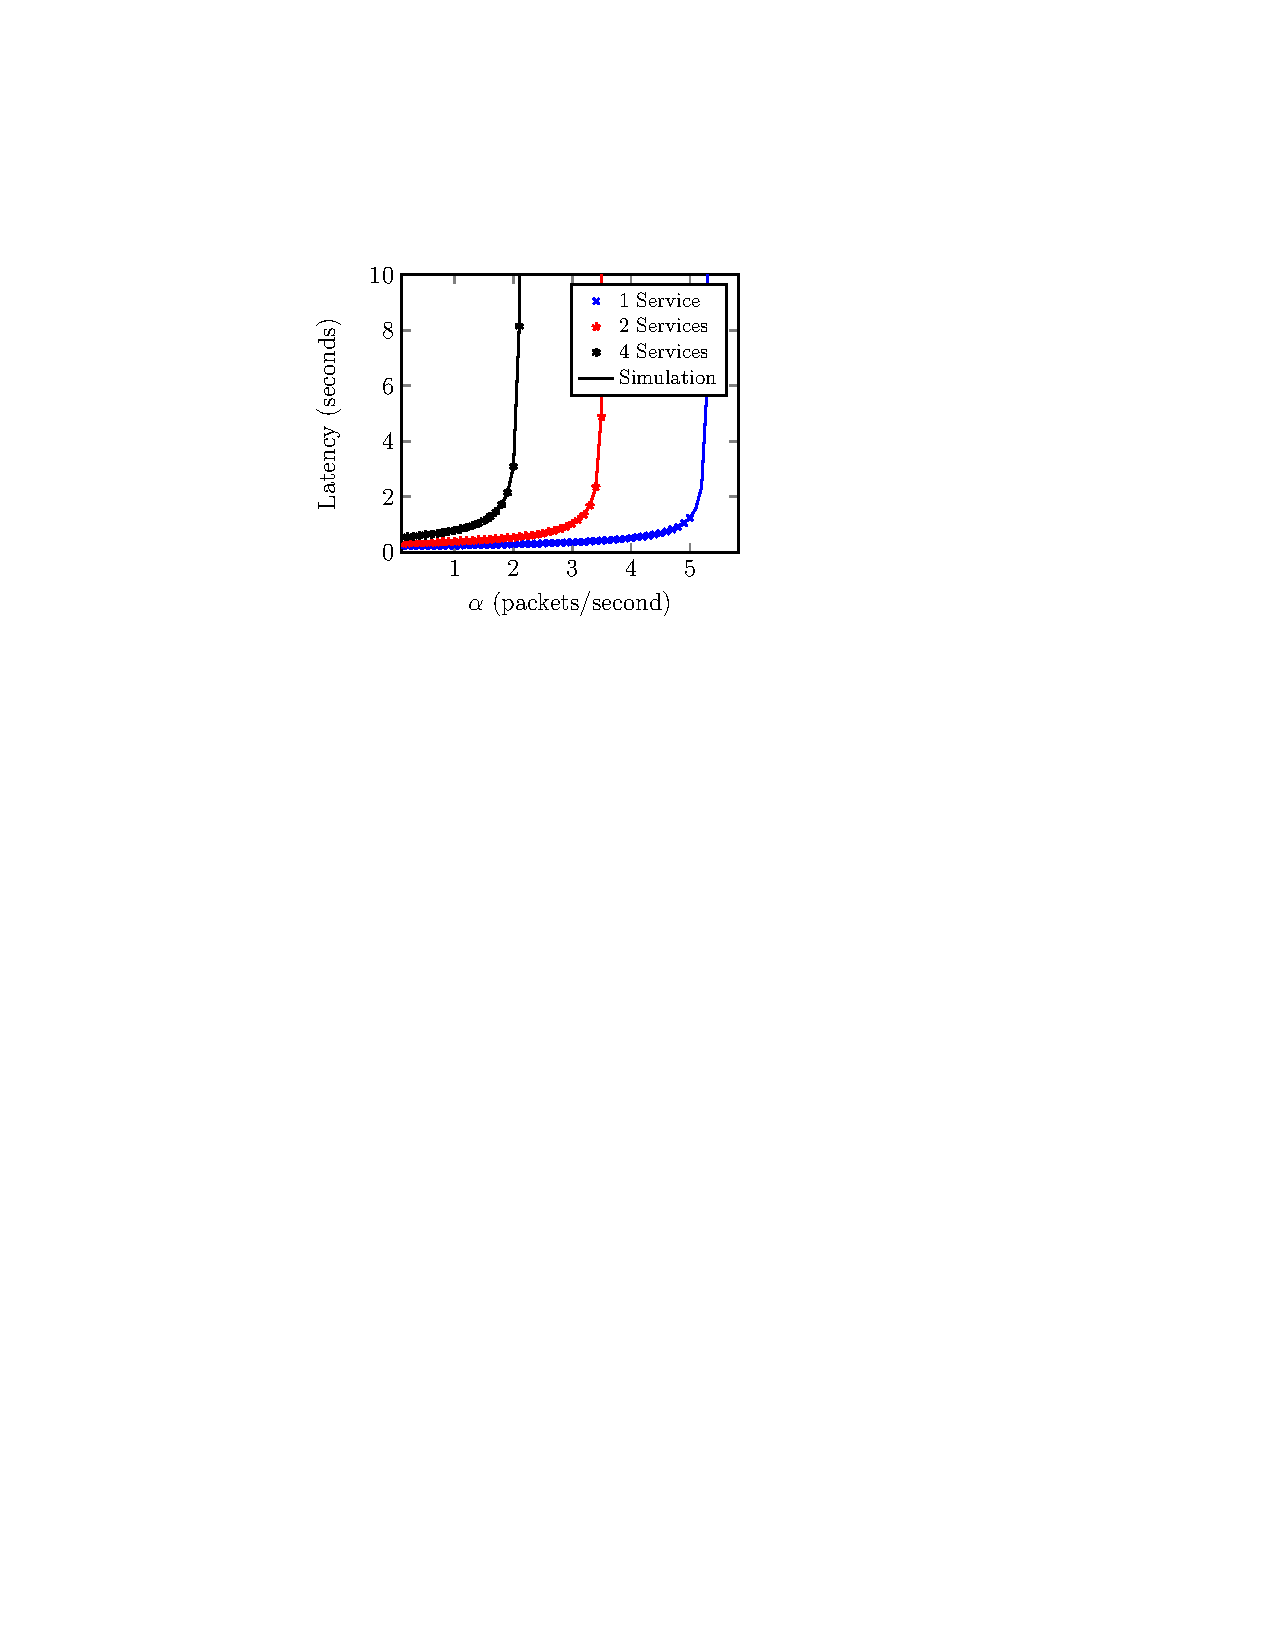
\includegraphics[width=\linewidth]{graphs/mult_services}
		\caption{Latency predicted by the model and simulation for several services ($N_s$)
			with different length service chains, $K_i = 2:(N_s+1)$.}
		\label{fig:mult_services}
	\end{minipage}

	\vspace{2mm}

	\centering
	\begin{minipage}[b]{.49\textwidth}
		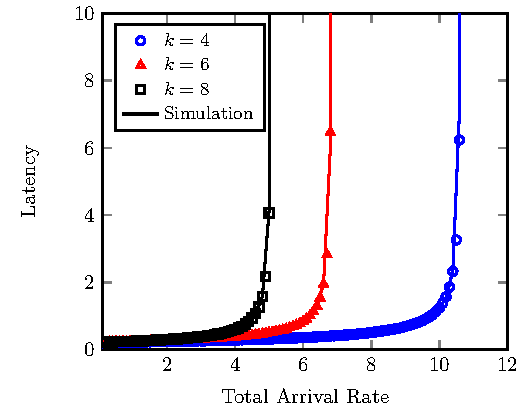
\includegraphics[width=\linewidth]{graphs/num_ports}
		\caption{Latency predicted by the model and simulation for different numbers
			of ports, $k$.}
		\label{fig:num_ports}
	\end{minipage}
	\hfill
	\begin{minipage}[b]{.49\textwidth}
		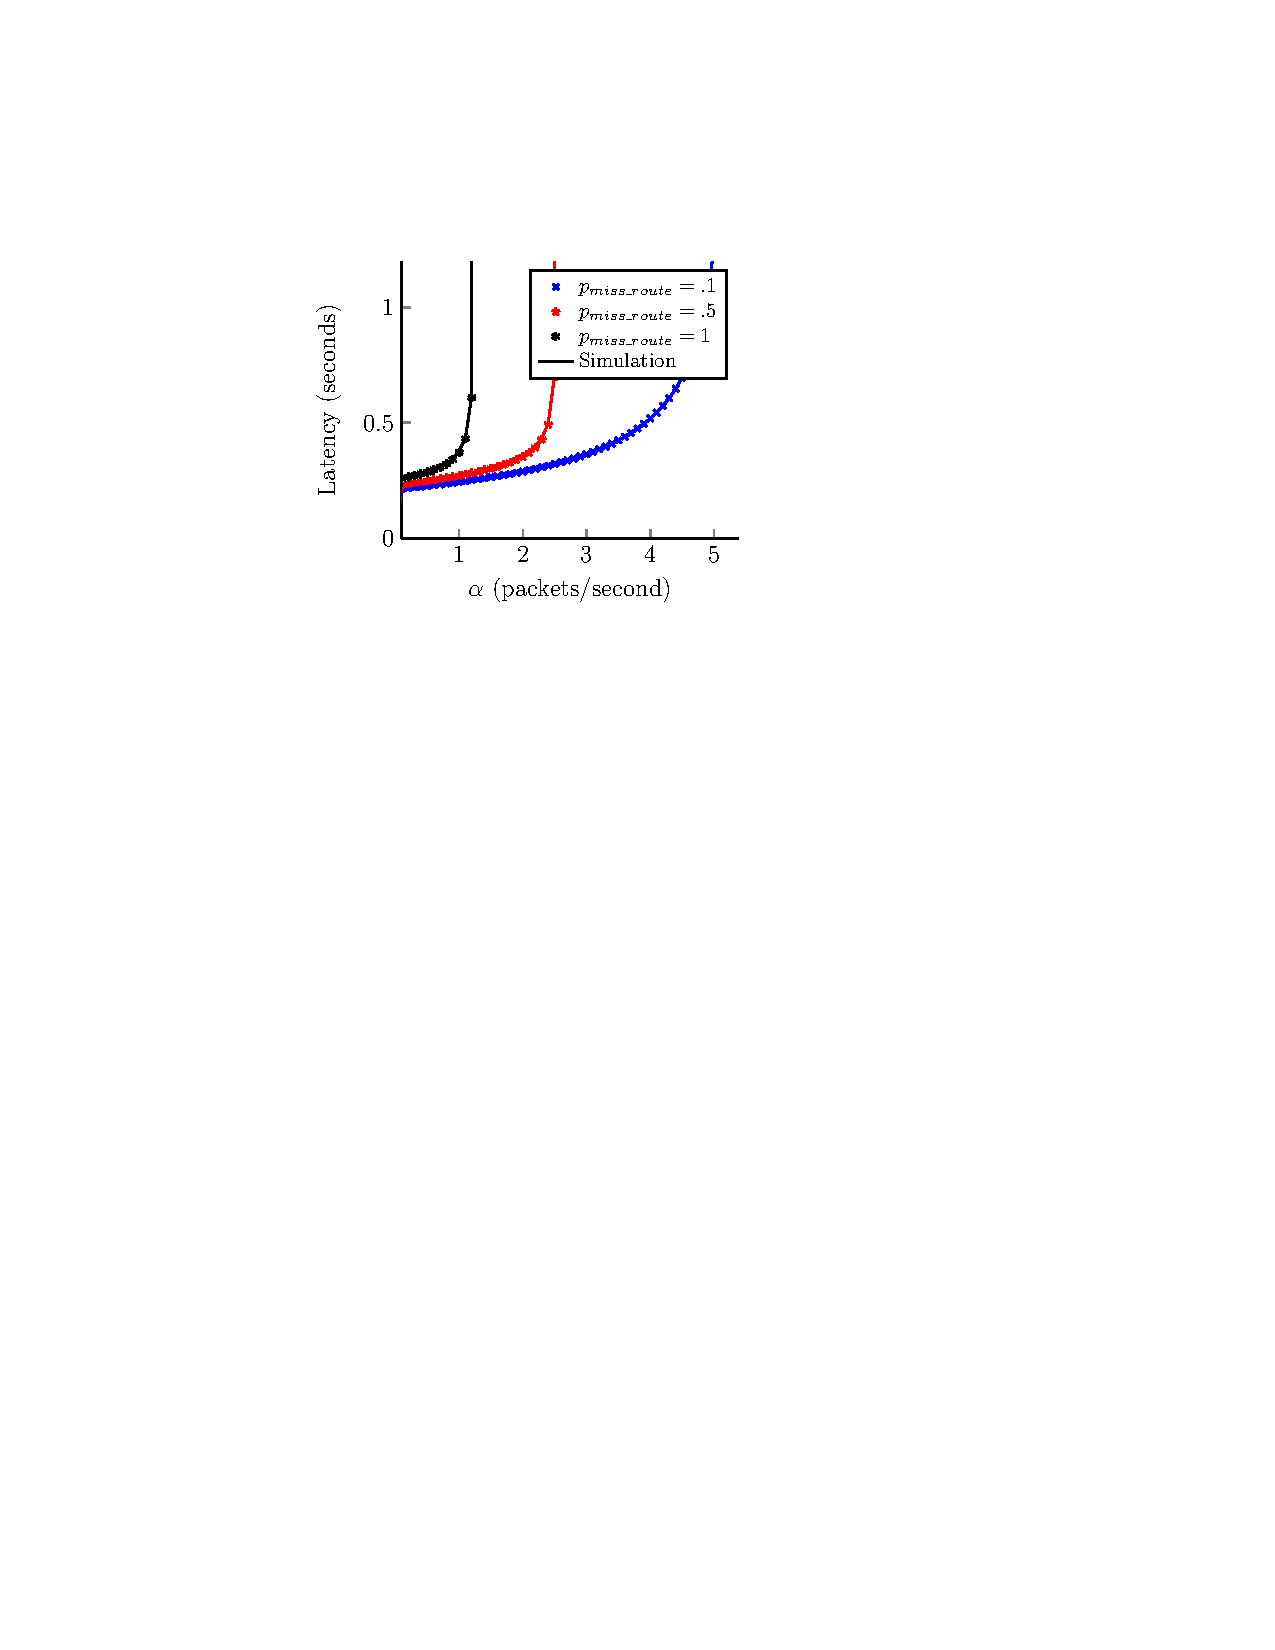
\includegraphics[width=\linewidth]{graphs/diff_sdn}
		\caption{Latency predicted by the model and simulation for different miss rates, $p_{m}$.}
		\label{fig:sdn_perc}
	\end{minipage}

\end{figure*}

\section{Validation and Performance Analysis}
\label{sec:validation}

\subsection{Validation}

To verify the accuracy of the analytical model, a discrete event simulator has been built using OMNeT++ \cite{VargaH08} to simulate a NFV and SDN enabled datacentre network. Each simulation experiment was run until the network reaches its steady state where further network cycles do not change the collected statistics appreciably. Comprehensive simulation experiments were conducted to validate the performance of the proposed analytical model under different network configurations. However for the sake of specific illustration only a selection of tests are presented here and the results comparison between the analytical model and simulation experiments are presented in terms of the average end-to-end latency.

In practice a datacentre can contain on the order of tens of thousands of servers \cite{AWS16}, with each switch supporting 1 to 100Gbits/s traffic a second. It is not feasible to simulate the scale of datacenter network in lab environment. Therefore, a scaled down version of a typical datacentre is modelled. Except where otherwise stated, the following parameters are used in our tests:

\begin{itemize}
	\item $k = \{4, 6, 8\}$, $k_{v} = 2$ and $p_{m} = \{0.1, 0.5, 1\}$
	\item The service rate of the switches and SDN controller are set to be 40 packets per second ($\mu_{v} = 40$, $\mu_{c} = 40$)
	\item The service rate of the VNFs is set to be 20 packets per second ($\mu_{f} = 20$)
	\item Services are selected with equal probability
	\item Case I: The network holds one service with two VNFs
	\item Case II: The network holds multiple services ($N_s = \{1,2,4\}$ and $K_i=\{3,5,7,9\}$)
	\end{itemize}
	
	Figs 2 to 5 depict mean message latency predicted by the model plotted against those provided by simulation experiments for a range of parameter settings. For the model, results are only shown where the network is in a steady state, i.e. where the arrival rate is lower than or equal to the service rate for all queues. The figures demonstrate that the simulation results closely match those predicted by the model. The tractability and accuracy of the analytical model make it suitable for analysis of next generation NFV and SDN enabled MCC datacentres.
	
	\subsection{Performance Analysis}
	After validating its accuracy, the proposed analytical model is used as a useful tool to optimise the system design for SDN and NFV enabled MCC datacenter network from the following three aspects, the number of the NFV services, the scale of the network infrastructure as well as the routing missing probability of SDN controller.
	
	\subsubsection{Impact of the number of NFV services on the end-to-end latency performance}
	
	As we all know that the datacenter network will be shared by multiple services to improve efficiency of the resource utilisation. So it is important to investigate of the end-to-end latency performance with the scenario of multiple NFV service deployment. From the Eq. (\ref{eq:effective_arrival}), multiple NFV deployment would result in higher traffic rates and longer waiting time for the packet delivery. From the Fig. 3, it can be seen that under the same arrival rate, e.g. $\lambda=3$, the end-to-end latency of the two services deployment is much larger than that of the one service deployment scenario. Further, with the increase of the number of VNFs in service chain, the waiting time increases greatly such that, as shown in Fig. 2, for services with length of 5 or above the system is only stable for proportionally low arrival rates. This can be observed from the Eq. (\ref{eq:latency_path}) that the longer service chain mean the packets would be processed by more VNFs and persist in the network longer, resulting in the worse end-to-end latency. Therefore, in the practical NFV service design, the long service chain should be avoid to obtain the lower transmission latency, through exploiting the technologies of NFV parallelisation design. 
	
	\subsubsection{Impact of the scale of datacenter network on the end-to-end latency performance}
	
	Modern datacenter could reach the scale of the hundreds of thousands of servers. When the SDN and NFV technologies are deployed in the datacenter network, it is necessary to investigate the scale of datacenter network on the performance of the end to end service provisioning.  The proposed analytical model could be used to quantitatively analyse this relationship. Under the same switch configuration, e.g. service rates on the edge, aggregation and core layers, the larger scale of datacenter infrastructure would lead to the higher end-to-end latency transmission. This is because for larger networks with a correspondingly larger number of VNFs the accumulated arrival rate at different layers causes the expected latency to increase even for small arrival rates. Counterintuitively, larger datacentres that are filled to capacity are not able to provide a better QoS than a smaller datacenter under the same conditions. From Eqs. (\ref{eq:p_vm} to \ref{eq:p_agg_core}) we can see this is a consequence of the high probability of packets going via higher layers of the datacentre for larger numbers of ports, hence overloading the higher layers as many packets must traverse all of the network layers. In a practical deployment, datacentre designers can adopt the strategy of placing nearby VNFs close with each other to reduce the transmission latency.
	
	\subsubsection{Impact of the missing rate of SDN flow table on the end-to-end latency performance}
	
	SDN paradigm provides the benefits of the simplified network management and the centralised system optimisation. However, from the packet forwarding perspective, the centralised control brings the extra transmission latency during packet delivery. The proposed analytical model allows us to investigate the relationship between the degree of the network centralised control and QoS performance of service provisioning. From the Fig. \ref{fig:sdn_perc} we can see that the end-to-end latency increases with the increase of the probability that a packet fails to match the flow table. This is because the higher value of $p_m$ leads to more packets to be sent to SDN controller. Considering Eq. \ref{eq:arr_sdn}, we can see that the arrival rate of the SDN controller is proportional to the network traffic that is produced by the VNFs. Due to the large connections from the virtual machine to SDN controller, even the slight increase of the traffic rate, $\lambda$, in the data plane, would result in the much higher traffic arriving at SDN controller. Therefore, to ensure that the SDN controller does not become a bottleneck for the end-to-end data transmission, network designers should ensure that the routing tables in the SDN controllers contain the majority of the information required so that few SDN requests are needed, or proactively increase the processing capability of SDN controller to handle huge amount of bustry requests from the virtual switches.